\documentclass{examen}

\begin{document}
\modulo{Lenguajes de marcas -- PARTE ESCRITA}


\pregunta{Haz una comparativa entre XML y HTML}{0.5}

\pregunta{
Una empresa desea modelar un flujo que indique las novedades en su canal de ventas, por lo que desea ver como quedar�a un archivo RSS que refleje dichas novedades.}{1.5}
\begin{itemize}
\item{La URL principal es http://acme.com y el canal de la empresa se llamar� ``Novedades de ACME'' siendo su descripci�n ``Las m�s recientes novedades al servicio de nuestros clientes''}
\item{Dentro de dicho canal se desea ver noticias de ejemplo}
\begin{enumerate}
	\item{La primera apunta a la URL http://acme.com/novedades1 su descripci�n es ``Disponible la nueva actualizaci�n de Android en los servidores de Google y r�plicas autorizadas`` y el t�tulo ``Nueva versi�n de Android''}
	\item{La segunda noticia tiene la URL http://acme.com/novedades2, su t�tulo es ``Fin de XP'' y la descripci�n es ``Finaliz� el soporte de Microsoft para Windows XP''}
\end{enumerate}

\end{itemize}




\pregunta{Elabora una p�gina web que contenga el formulario siguiente:}{3}
\begin{itemize}

\item{    Contiene los siguientes radiobuttons:radio con el name ``mediotransporte'' , value ``mediotransporteautomovil'' y el texto ``Autom�vil'', radio con el name ``mediotransporte'' , value ``mediotransportemoto'' y el texto ``Moto'', radio con el name ``mediotransporte'' , value ``mediotransporteautobus'' y el texto ``Autob�s''.}
\item{    Hay un textarea que mide 6 filas y 47 columnas que lleva dentro el texto ``Utilice este recuadro por favor''}
\item{    Contiene los siguientes checkboxes:checkbox con el name ``formato'' , value ``formatojpg'' y el texto ``JPG'', checkbox con el name ``formato'' , value ``formatopng'' y el texto ``PNG''.}

 
\end{itemize}
\begin{figure}
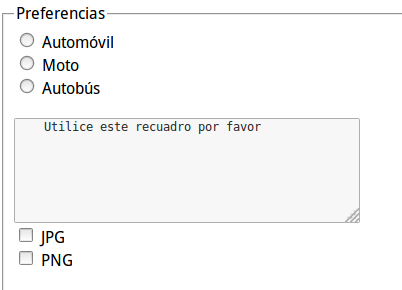
\includegraphics[scale=0.7]{examen-img/foto_formulario_14.png}
\end{figure}
\end{document}

